\title{%
  A Science of Security Course: An Overview
}
\author{Daniel Bosk\thanks{%
    This material was authored by Daniel Bosk and is available under the 
    Creative Commons Attribution-ShareAlike (CC-BY-SA) 4.0 international 
    license.
}}
\institute{%
  KTH EECS, \email{dbosk@kth.se}
}

\mode<article>{\maketitle}
\mode<presentation>{%
  \begin{frame}
    \maketitle
  \end{frame}
}

\mode*

\begin{abstract}
  \mode*

% What's the problem?
% Why is it a problem? Research gap left by other approaches?
% Why is it important? Why care?
% What's the approach? How to solve the problem?
% What's the findings? How was it evaluated, what are the results, limitations, 
% what remains to be done?

% XXX Summary
\emph{Summary:}
In this learning session we will give an introduction to the scientific method 
and particularly how this can be applied in the area of security.

% XXX Motivation and intended learning outcomes
\emph{Intended learning outcomes:}
After this session you should be able:
\begin{itemize}
  \item to \emph{apply} the scientific method correctly to answer basic 
    questions in security.
\end{itemize}

% XXX Prerequisites
%\emph{Prerequisites:}
%\dots

% XXX Reading material
\emph{Reading:}
You should read 
\citetitle{HowToDesignSecurityExperiments}~\cite{HowToDesignSecurityExperiments}.
This paper discusses the scientific method of (parts of) the security field.
For a more in-depth reflection on the state of security as a scientific pursuit, 
we recommend
\citetitle{SecurityAsAScience}~\cite{SecurityAsAScience}.

\end{abstract}

\clearpage
\tableofcontents
\clearpage

\section{Overview}

\only<presentation>{\subsection{The goal}}

The goal of the course is to give a holistic view of the Science of Security.
We want to answer the following question:

\begin{frame}
  \begin{question}
    What are the methods we (in the security community) use and why?
  \end{question}
\end{frame}

\begin{frame}<presentation>
  \begin{block}{The goal}
    \begin{itemize}
      \item Give a holistic view of Science of Security.
      \item What are the methods we use and why?
    \end{itemize}
  \end{block}
\end{frame}

This is a tricky question to answer, because there are some apparent problems 
with the scientificity in the security area.
Consider the following examples.

\begin{frame}[fragile]
  \begin{example}\label{SoKProblem1}
      \textcquote[\S IV]{SecurityAsAScience}{\textins*{C}laims of necessary 
        conditions for real-world security are unfalsifiable.
      Claims of necessary conditions for formally-defined security are 
    tautological restatements of the assumptions}.
  \end{example}

  \pause

  \begin{example}\label{SoKProblem2}
    \textcquote{SecurityAsAScience}{%
      Unfalsifiable claims are common in security---and they, along with circular 
      arguments, are used to justify many defensive measures \textelp{}
      \textins{T}here are many ways to argue measures in, but no way to argue one 
      out.
    }
  \end{example}
\end{frame}

This leads us to the second question, we want the students to able to answer:

\begin{frame}
  \begin{question}
    What makes my work (in security) scientific?
  \end{question}
\end{frame}

\begin{frame}<presentation>
  \begin{block}{Aim of Science of Security course}
    \begin{itemize}
      \item Complement the general methods course.
      \item Better prepare students for thesis (and hopefully worklife \dots).
      \item They should be able to contribute to scientifically based 
        development in cybersecurity.
    \end{itemize}
  \end{block}
\end{frame}

\only<article>{\subsection{Goals and requirements}}

Now the aim of the course is to complement the general scientific methods 
course.
Due to the complexity of security problems and the field's interdisciplinary 
composition, we want to emphasise on how the methods fit together in the field.
We find this particularly necessary after reading the quotes in 
\cref{SoKProblem1,SoKProblem2}.

The requirements for Master's level are set out in 
\citetitle{HEO2}~\autocite{HEO2}, namely:
\begin{frame}[fragile]
  \begin{block}{Master's goals: Knowledge and understanding~\autocite{HEO2}}
    \only<article>{\begin{enumerate}[label={(K\arabic*)},ref=K\arabic*]}
    \only<presentation>{\begin{itemize}}
      \item\label{K1} demonstrate knowledge and understanding \textelp{} as 
        well as insight into current research and development work, and
      \item\label{K2} demonstrate specialised methodological knowledge in the 
        main field of study.
      \item\label{K3} demonstrate the ability to critically and systematically 
        integrate knowledge and analyse, assess and deal with complex 
        phenomena, issues and situations even with limited information
    \only<article>{\end{enumerate}}
    \only<presentation>{\end{itemize}}
  \end{block}
\end{frame}

\begin{frame}[fragile]
  \begin{block}{Master's goals: Competence and skills~\autocite{HEO2}}
    \only<article>{\begin{enumerate}[label={(C\arabic*)},ref=C\arabic*]}
    \only<presentation>{\begin{itemize}}
      \item\label{C1} demonstrate the ability to identify and formulate issues 
        critically, autonomously and creatively as well as to plan and, using 
        appropriate methods, undertake advanced tasks
        \only<presentation>{\textelp{}}%
        \only<article>{within predetermined time frames}
        and so contribute to the formation of knowledge as well as the ability 
        to evaluate this work
      \item\label{Ccomm} demonstrate the ability in speech and writing both 
        nationally and internationally to clearly report and discuss his or her 
        conclusions and the knowledge and arguments on which they are based in 
        dialogue with different audiences, and
      \item\label{C2} demonstrate the skills required for participation in 
        research and development work \textelp{}
    \only<presentation>{\end{itemize}}
    \only<article>{\end{enumerate}}
  \end{block}
\end{frame}

\begin{frame}[fragile]
  \begin{block}{Master's goals: Judgement and approach~\autocite{HEO2}}
    \only<article>{\begin{enumerate}[label={(J\arabic*)},ref=J\arabic*]}
    \only<presentation>{\begin{itemize}}
      \item\label{J1} demonstrate the ability to make assessments in the main 
        field of study informed by relevant disciplinary, social and ethical 
        issues and also to demonstrate awareness of ethical aspects of research 
        and development work
      \item\label{J2} demonstrate insight into the possibilities and 
        limitations of research, \textelp{}
    \only<presentation>{\end{itemize}}
    \only<article>{\end{enumerate}}
  \end{block}
\end{frame}

\paragraph{Intended learning outcomes}\label{LearningOutcomes}

\begin{frame}[fragile]
  \only<article>{In summary, the learning outcomes, we want that after}%
  \only<presentation>{After}%
  passing the course, the student should be able to
  \only<article>{\begin{enumerate}[label={(LO\arabic*)},ref=LO\arabic*]}
  \only<presentation>{\begin{itemize}}
    \item\LOrelate{}
      \only<article>{[\ref{K1}, \ref{K2}, \ref{J2}]}
    \item\LOevaluate{}
      \only<article>{[\ref{C1}, \ref{C2}, \ref{J1}, \ref{K3}]}
    \item\LOapply{}
      \only<article>{[\ref{C1}, \ref{C2}]}
    \only<presentation>{%
    \item \dots
    }
    \only<article>{%
    \item\LOplan{}
      \only<article>{[\ref{C1}]}
    \item\LOcomm{}
      \only<article>{[\ref{K3}, \ref{Ccomm}]}
    }
  \only<presentation>{\end{itemize}}
  \only<article>{\end{enumerate}}
  in order to be able to contribute to scientifically based development.
\end{frame}

\subsection{Prerequisites}

The course requires some prerequisites.
In the area of cybersecurity, the student should be able to:
\begin{itemize}
  \item identify threats against confidentiality, integrity and availability in 
    digital systems
  \item explain basic terminology and concepts in computer security and use 
    them
  \item find and use documentation of security related problems and tools
  \item analyse simple program code and systems (based on given or self-made 
    system descriptions) to identify vulnerabilities and predict corresponding 
    threats
  \item select countermeasures against identified threats and argue for their 
    suitability
  \item compare countermeasures and evaluate their side effects,
  \item apply countermeasures present and explain their reasoning to others.
\end{itemize}

In the area of the cybersecurity engineer's role in society, the student should 
be able to:
\begin{itemize}
  \item analyse and discuss how the use and development of digital systems and 
    in particular the security of these systems affect and are affected by 
    social, economic, environmental, work environmental and ethical 
    sustainability as well as diversity, gender equality and equal conditions
  \item review critically and reflect on both the set-up and implementation of 
    the education as well as their own study situation, their skills in 
    relation to the objective of the education and the future professional role 
    and their ability to identify their own need of additional knowledge
  \item plan and carry out assignments within given time frames and using 
    available resources
  \item write short, clear and arguing texts based on own analysis as well as 
    given material.
\end{itemize}

Finally, since course is intended to complement the general research methods 
course, we expect the students to, with regards to the theory and  methodology 
of science, both orally as well as in writing, be able to:
\begin{itemize}
  \item identify definitions and descriptions of concepts, theories and problem 
    areas, as well as identify the correct application of these concepts and 
    theories;
  \item account for concepts, theories and general problem areas, as well as 
    apply concepts and theories to specific cases;
  \item critically discuss the definitions and applications of concepts and 
    theories as they applies to specific cases of scientific research.
\end{itemize}


\section{More concretely}

Let's return to the goal of the course and then proceed to its contents.

\subsection{The goal}

Let's have a look at provable security, widely considered the epitome of 
security research.

\begin{frame}<presentation>
  \begin{example}[\enquote{Provable security}]
    \begin{itemize}
      \item A uniformly random string of length \(n\) is the most secure 
        password.

      \item We can prove it will take millions of years to guess it.
    \end{itemize}
  \end{example}

  \pause

  \begin{remark}
    \begin{itemize}
      \item Attackers still get in, weird \dots
    \end{itemize}
  \end{remark}
\end{frame}

\begin{example}[\enquote{Provable security}]\label{SecurePassword}
  A uniformly random string of length \(n\) is the most secure password.
  We can prove it will take millions of years to guess it.
\end{example}

\begin{frame}<presentation>
  \begin{example}[Usability]
    \begin{itemize}
      \item Turns out people can't handle uniformly random passwords.
      \item Particularly not with a unique such password for every service.
      \item They can't generate uniformly random passwords either.
    \end{itemize}
  \end{example}

  \pause

  \begin{remark}[Several aspects]
    \begin{itemize}
      \item We want students to handle complex problems.
      \item Should see there are several aspects.
      \item Aspects must be approached differently.
    \end{itemize}
  \end{remark}
\end{frame}

However, attackers still get in.
% XXX add refs to password literature
It turns out that humans can't handle long, uniformly random passwords.
Particularly not when they have to remember one such password \emph{per service 
they use}.
And they can't generate uniformly random passwords either!
None of these results could be found through provable security, they're from 
the usability area of security and the methods are from the usability and 
human--computer interaction research field.

By this we don't say that provable security is wrong or doesn't work.
The same can be said of the usability methods.
Both are needed, they complement each other in generating understanding of 
security problems.
The goal of the course is that the students should be able to master the 
variety of methods [\ref{LOrelate}] and combine them to answer questions about 
security problems [\ref{LOapply}].
That includes being able to evaluate different approaches to answering 
questions and choosing among the most suitable ones [\ref{LOevaluate}].

Knowledge dissemination is about communicating results to others.
And in science, to convince others that one's results are correct.
We can see this aspect in \ref{LOcomm} (and \ref{Ccomm}) and we will see this 
aspect as part of the assessment of the course later.


\subsection{Teaching design}

The teaching design of the course is particularly interesting to describe in 
this course, because it is highly relevant on the meta level.

\begin{frame}<presentation>[fragile]
  \begin{block}{Teaching design}
    \begin{itemize}
      \item Have problems that must be explored using several 
        methods.
      \item Work through enough problems to cover the entire spectrum.
    \end{itemize}
  \end{block}

  \begin{remark}[Learning theory]
    \begin{columns}[T]
      \begin{column}{0.6\columnwidth}
          \centering
          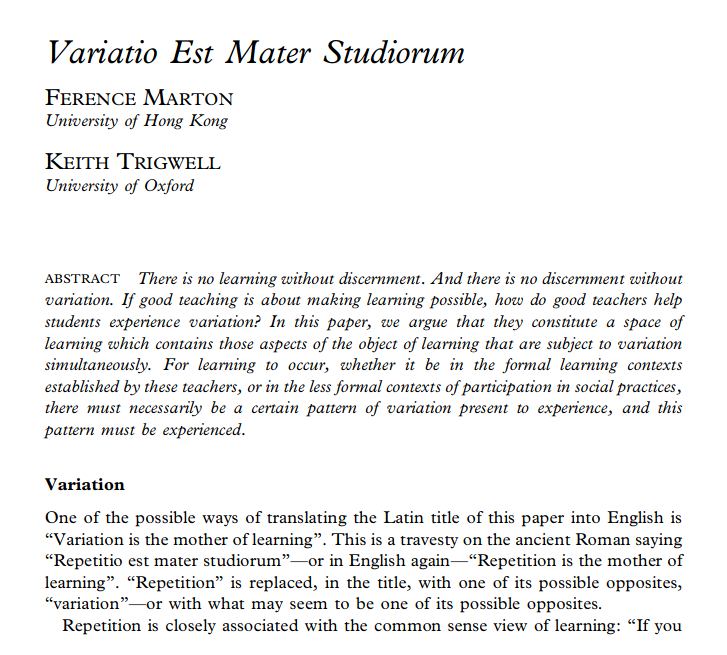
\includegraphics[width=0.8\columnwidth]{figs/variatio-mater-studiorum.png}
        \end{column}
        \begin{column}{0.4\columnwidth}
          
\includegraphics[height=0.55\textheight]{figs/NCOL.jpg}
        \end{column}
      \end{columns}
  \end{remark}
\end{frame}

The design of the course is based on the variation theory of learning~\cite[see 
\eg][]{NecessaryConditionsOfLearning}.
The goal of the theory is to achieve learning that prepares for unknown 
situations.
It aims for deep learning (as opposed to surface learning, 
\cf~\cite{DeepSurfaceLearning}).
This fits very well with our learning outcomes (\cref{LearningOutcomes}).
In fact, \textcite{NecessaryConditionsOfLearning} makes a point that learning 
(according to this theory), is in fact very aligned with science and research.
However, variation theory, according to me, tells us more than the scientific 
method traditionally does; it tells us about the preconditions to scientific 
discovery.

But what does this mean for the course concretely?
Well, in a sense, we could say that the teaching will treat some situations and 
the assessment will treat something \enquote{completely different}.
Of course, there is something in common, namely the essence of the course.
But the purpose of the assessment is to test if the student can use what 
they've learned from the teaching to handle this unknown situation---because 
that's what the thesis and the rest of their careers are about.
Now this also means that if a student adopts the approach of opening the 
assignments and then try to find the correct answers in the teaching material, 
that student will be very disappointed in the course.

In essence, we will look at problems and work out suitable methods to answer 
questions about the problem at hand.
(This is the pattern of variation called contrast, in terms of 
\cite{NecessaryConditionsOfLearning}, and focuses on \ref{LOrelate}, it's the 
first and crucial step of learning.)
Then we'll dive into each method to explore what kinds of questions it can help 
answer.
(This is the pattern of variation called generalization, in terms of 
\cite{NecessaryConditionsOfLearning}, and focuses on \ref{LOevaluate}.
Coincidentally, this pattern corresponds to what is called the scientific 
method.)
Finally, we will combine the methods to answer more complex questions.
(This is the variation of fusion, in terms of 
\cite{NecessaryConditionsOfLearning}, and focuses on \ref{LOapply}.)
The assessment will then be a new problem where the students must combine the 
methods to answer more complex questions on their own.

For the remaining learning objectives, \ref{LOplan} and \ref{LOcomm}, we will 
use the students' own works as learning material.
The idea is as follows:
The students will review each others' works, so this concerns \ref{LOcomm}.
If the work is about arguing why a method answers a particular research 
question, then another student's solution will provide a contrasting 
perspective to one's own.
Even if the choice of method is the same, the phrasing of the arguments 
provides contrast to one's own arguments and phrasing thereof.

We allow for \ref{LOplan} by giving the teaching material, assignments and 
their deadlines for participating in seminars in advance.
Since the course runs in every period, it's up to the student to make a plan 
for when to complete the assignments and participate in the seminars.
It's fine if a plan needs adapting, life happens; the important thing is that 
the students learn to deal with it.
The assessment of this learning outcome consists of evaluating the plan, how it 
turned out and what the student learned.

\subsection{Format}

We have the following division of credits in LADOK\footnote{%
  See the syllabus:
  \url{https://www.kth.se/student/kurser/kurs/DA2215?l=en}.
}\footnote{%
  There is a similar line in DD2302.
}:
\begin{description}
  \item[INL1] Seminars and assignments, 3.0 credits, grading scale: P, F
\end{description}

The assignments consists of reading and social annotation in an online tool 
(\cref{fbfdocquiz,fbfdocannotation}).
The seminars are live seminars on Zoom (or in-person on campus).
The idea is that you learn from the first few seminars, so that we can grade 
you on the last one.

\begin{figure}[t]
  \begin{fullwidth}
  \subbottom[%
  An interactive document in FeedbackFruits where one can answer quiz questions 
  posed in the document and ask questions about the content.%
  \label{fbfdocquiz}%
  ]{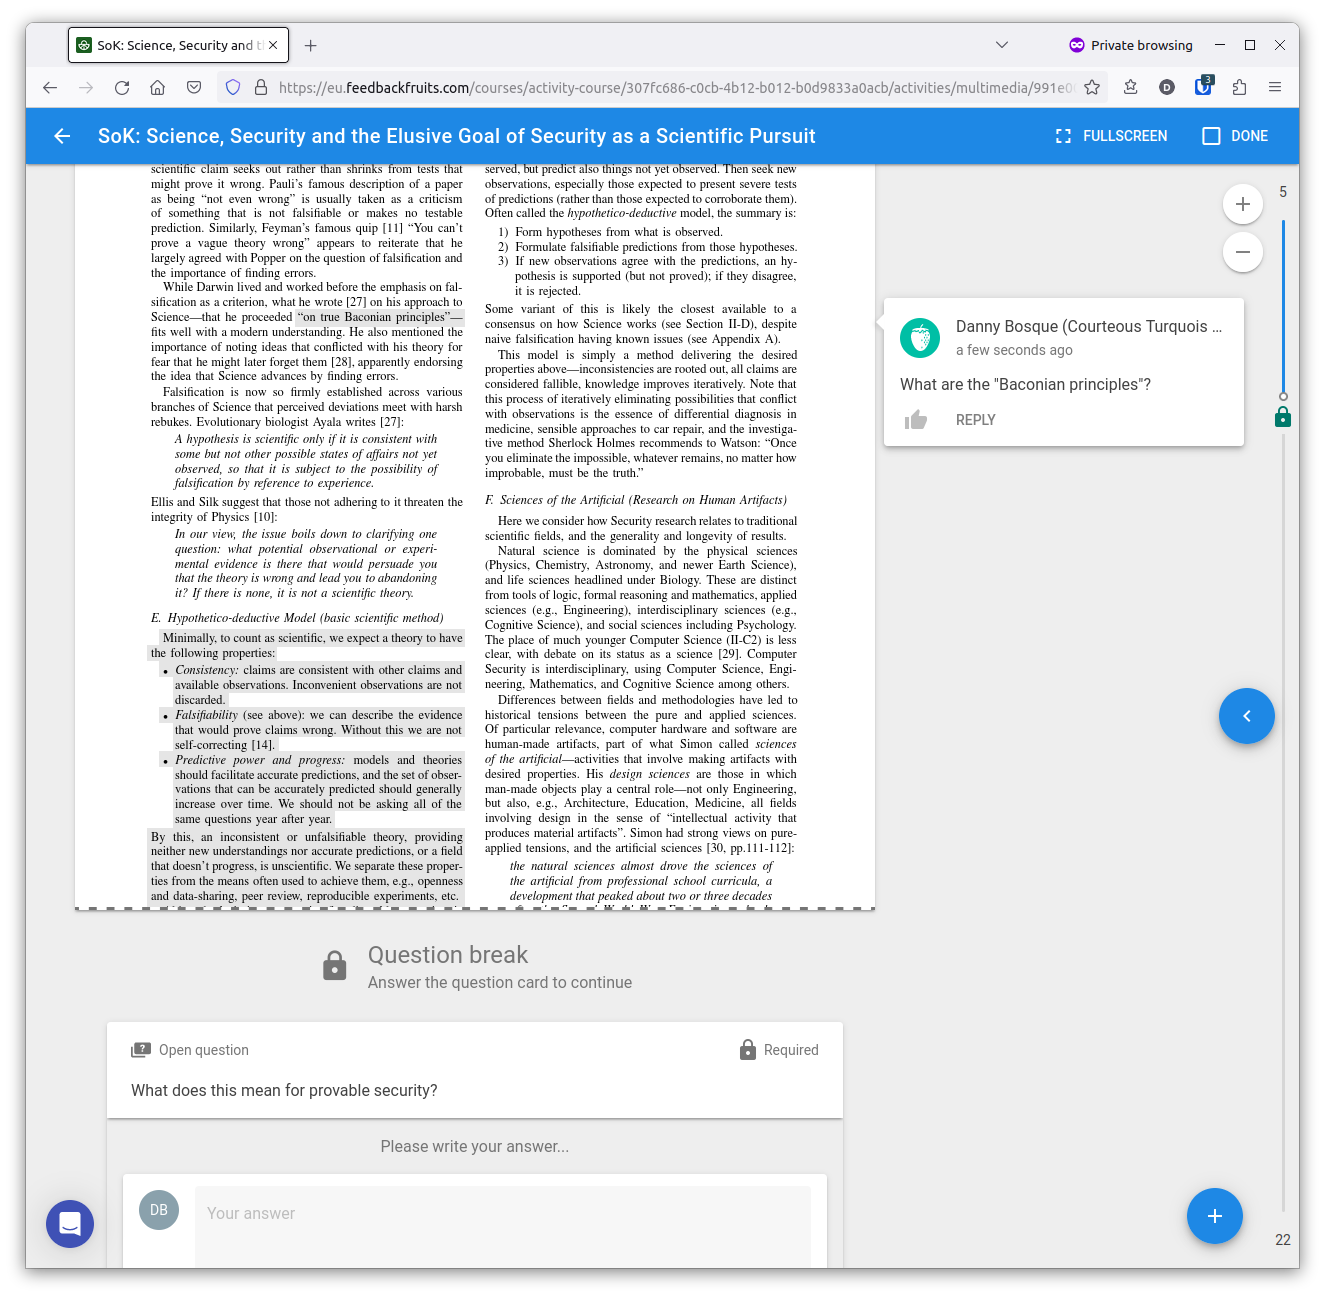
\includegraphics[height=0.3\textheight]{figs/fbf-doc-quiz-question.png}}
  \hspace{1em}
  \subbottom[%
    An interactive document in FeedbackFruits where one can annotate the text 
    with focused topics together with other students in the class.%
    \label{fbfdocannotation}%
  ]{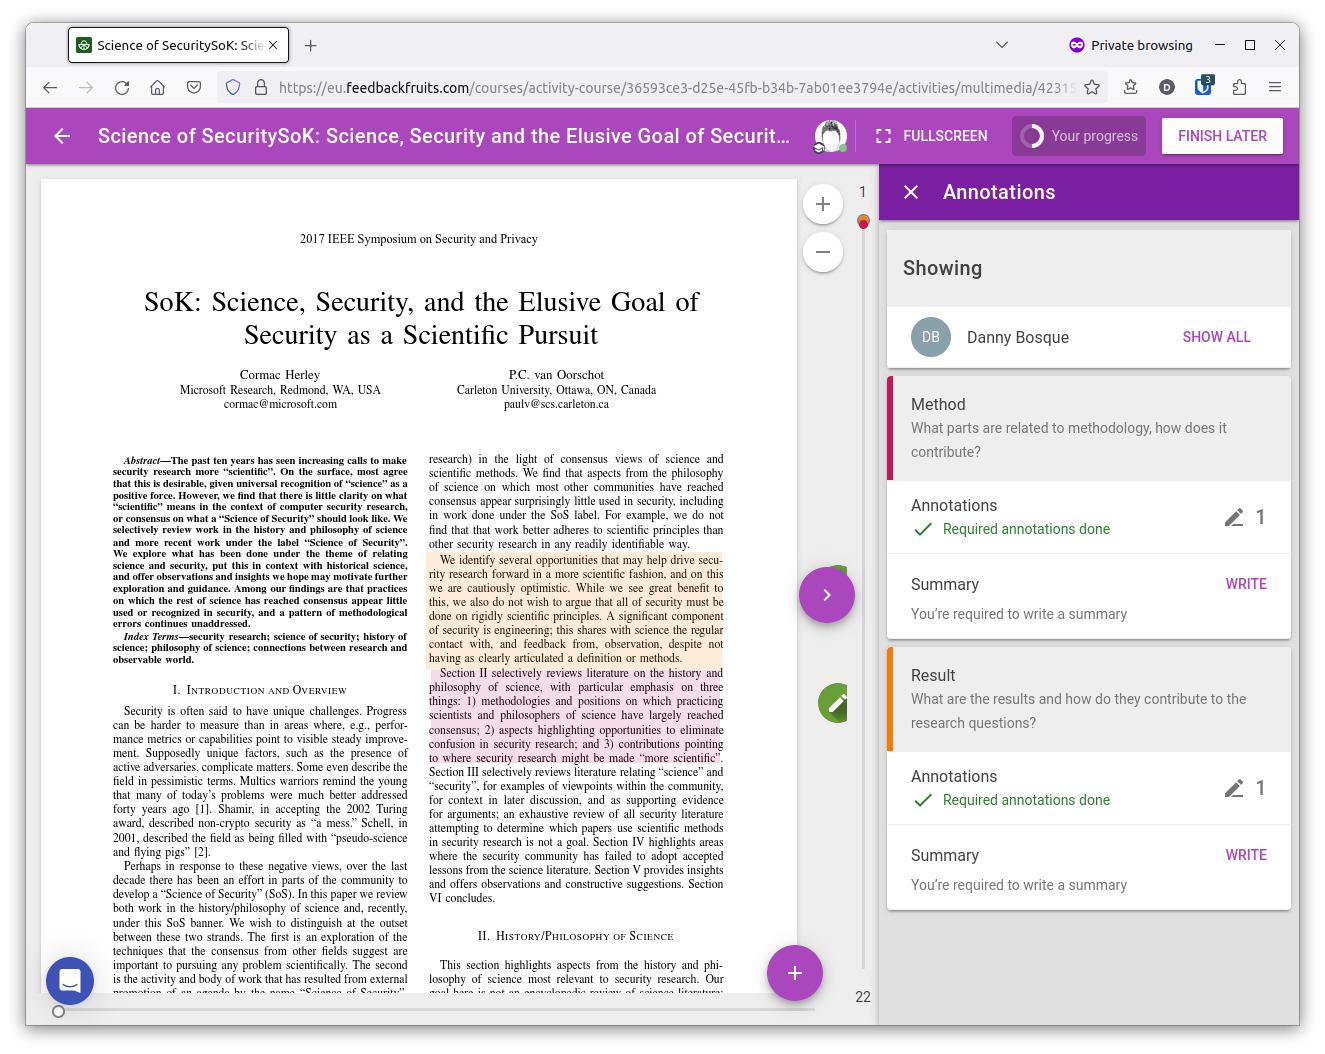
\includegraphics[height=0.3\textheight]{figs/fbf-doc-annotations.png}}
  \caption{Two ways of having interactive documents.}\label{fbfdoc}
  \end{fullwidth}
\end{figure}

\mode<presenation>{%
\begin{frame}[fragile]
  \begin{block}{Examination}
    \begin{description}
      \item[INL1] Seminars and assignments, 3.0 credits, grading scale: P, F
    \end{description}
  \end{block}

  \pause

  \begin{block}{Format}
    \begin{itemize}
      \item Online assignments
      \item Asynchronous, social annotation
      \item One final seminar, online or in-place
    \end{itemize}
  \end{block}
\end{frame}
}

The reading assignments are part of the learning material.
These are complemented by interactive video lectures (\cref{fbfvideo}) and the 
early seminar sessions.
In the video lectures the students can ask questions and answer quizzes.
The seminar sessions (not the last one) aim at exploring the paths not taken in 
the material.

\begin{marginfigure}
  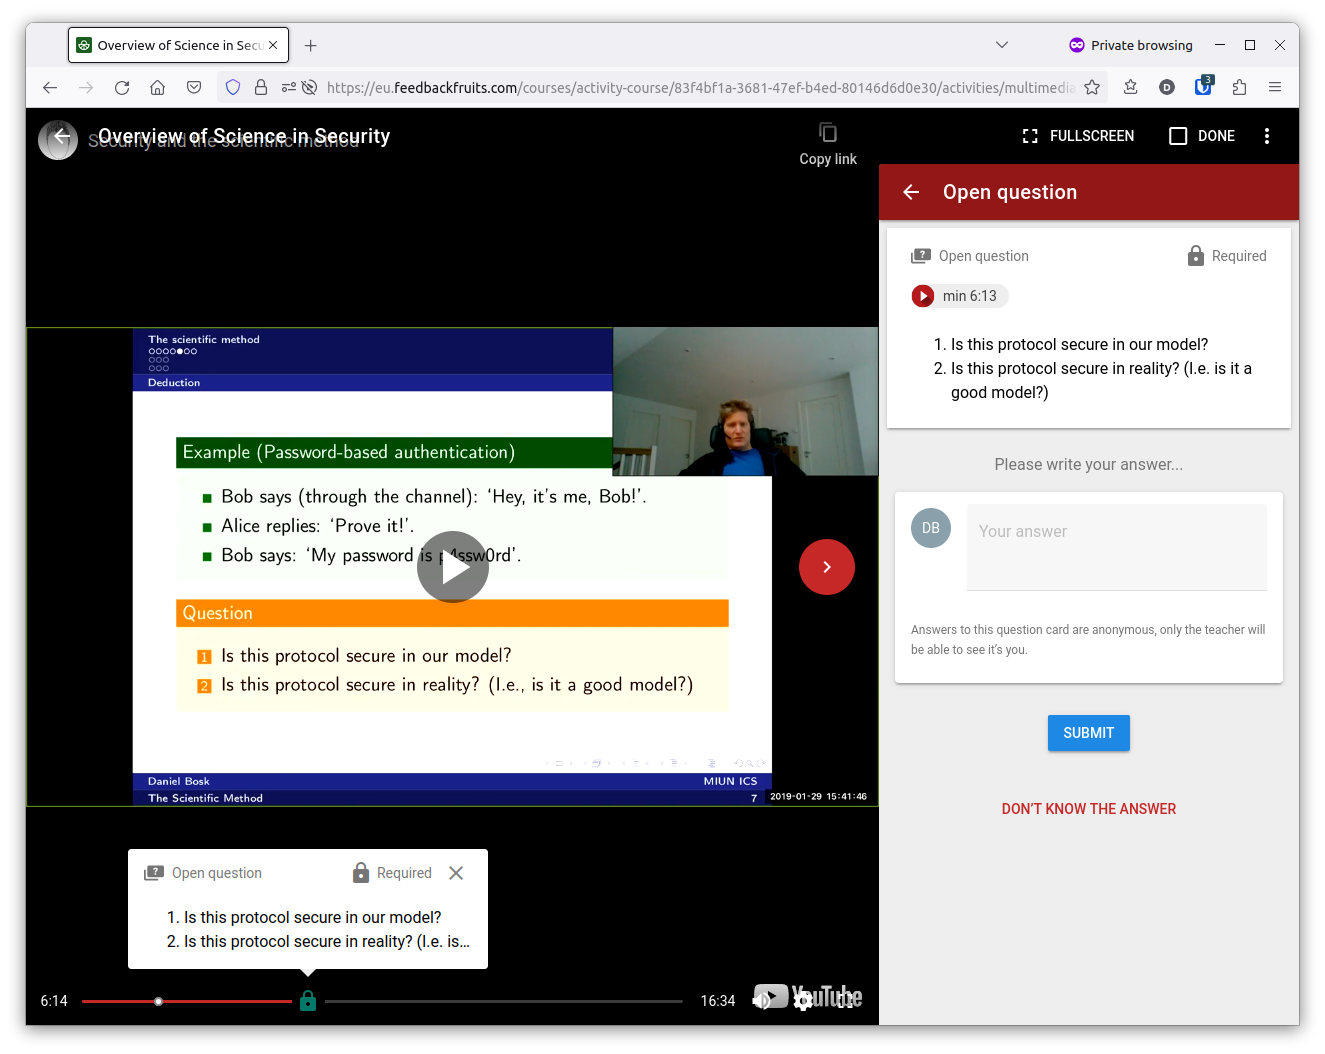
\includegraphics[width=\columnwidth]{figs/fbf-video-quiz.png}
  \caption{%
    An interactive video in FeedbackFruits where one can answer quiz 
    questions posed in the video.%
  }\label{fbfvideo}
\end{marginfigure}


\mode<presentation>{%
\begin{frame}
  \begin{columns}
    \begin{column}{0.5\columnwidth}
      \begin{block}{Teaching material}
        \begin{itemize}
          \item<1> Video lectures where students can ask questions and answer 
            quizzes\footnote{FeedbackFruits or Canvas Studio}.

            \pause

          \item<2-3> Reading assignments with social annotation\footnote{%
              FeedbackFruits or Perusall
            }.
        \end{itemize}
      \end{block}
    \end{column}
    \begin{column}{0.5\columnwidth}
      \only<1>{
        \begin{figure}
          \centering
          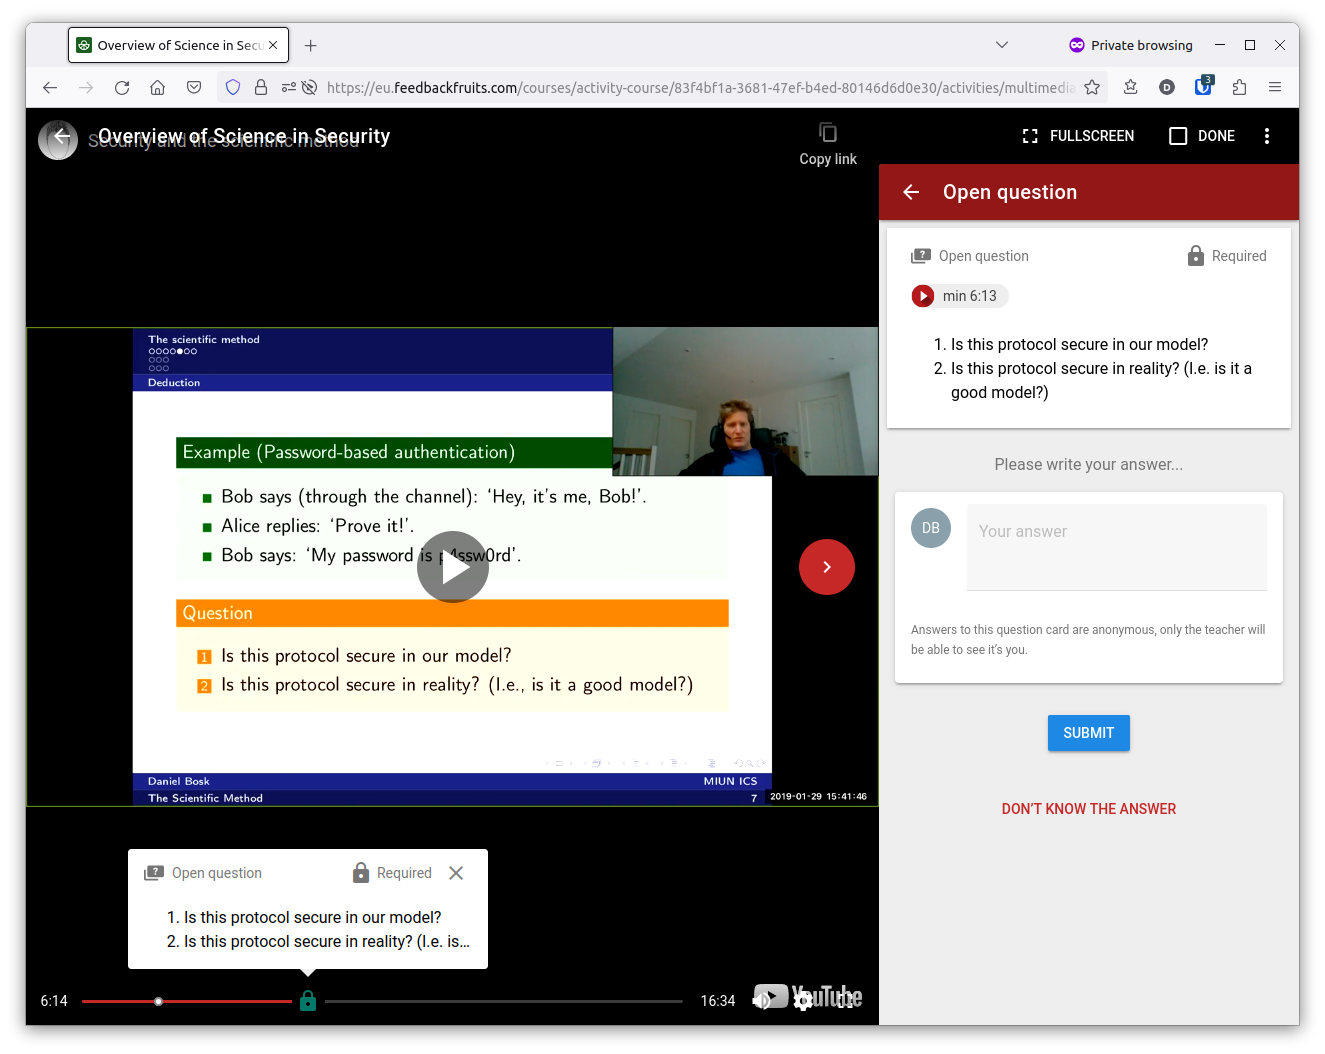
\includegraphics[width=\columnwidth]{figs/fbf-video-quiz.png}
          \caption{%
            An interactive video in FeedbackFruits where one can answer quiz 
            questions posed in the video.%
          }
        \end{figure}
      }
      \only<2>{
        \begin{figure}
          \centering
          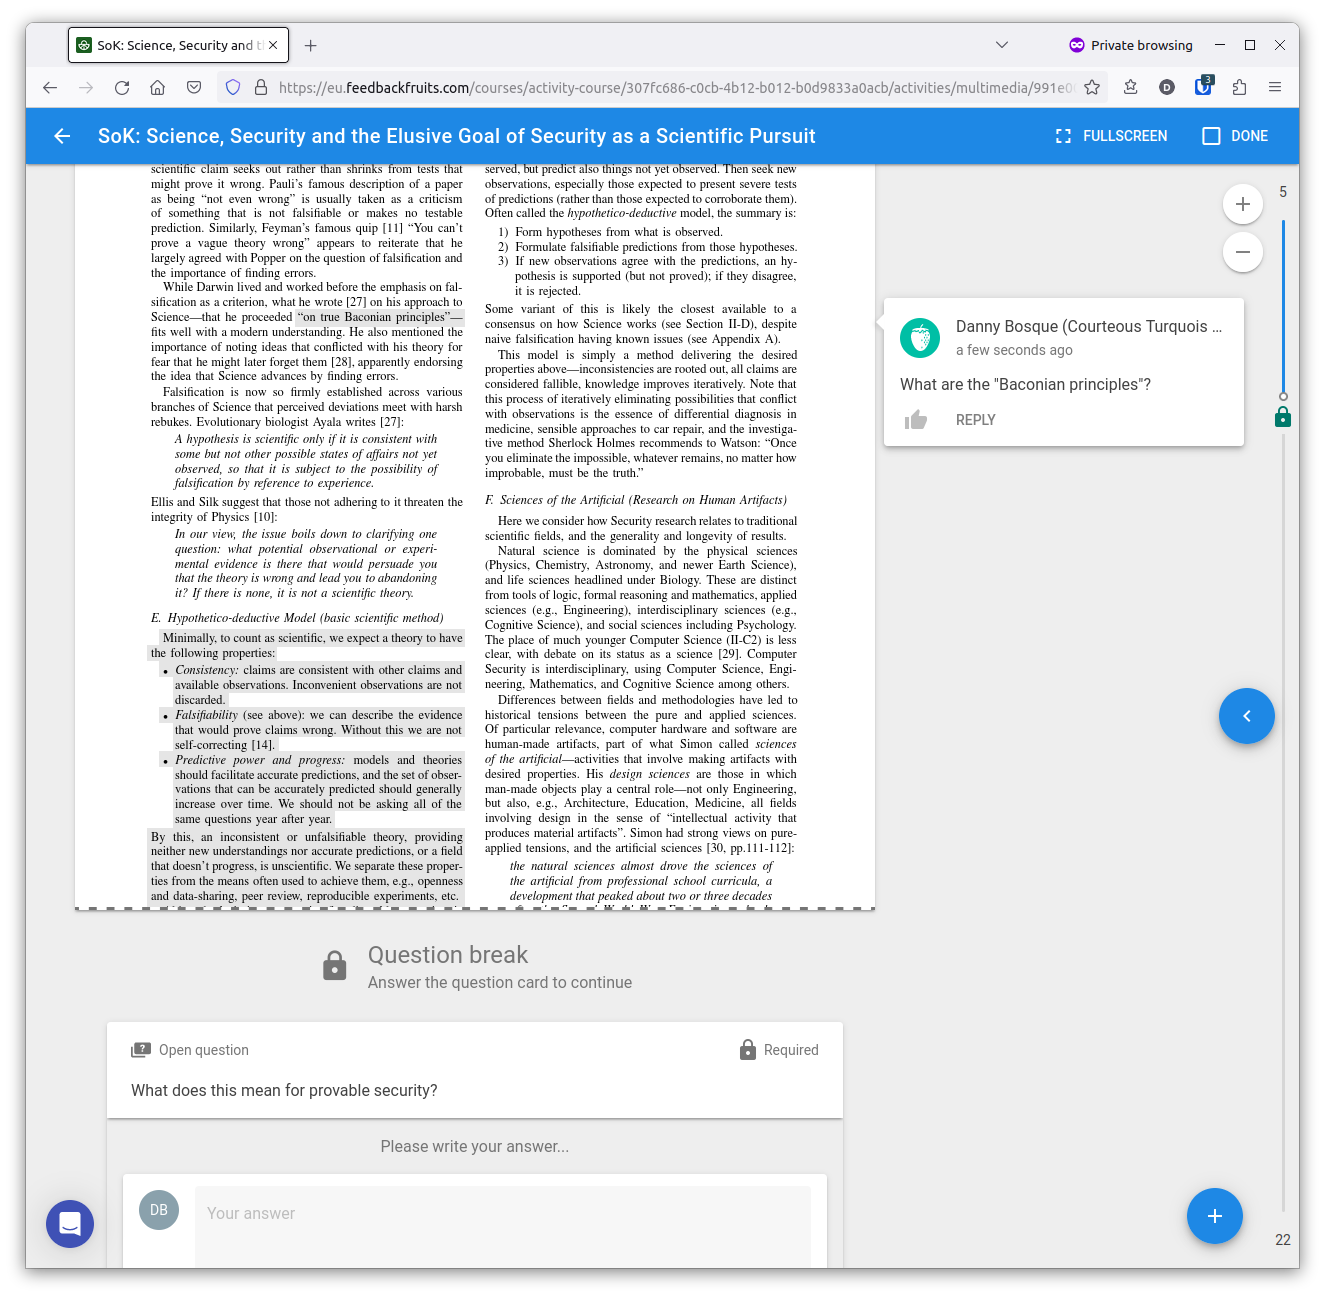
\includegraphics[width=\columnwidth]{figs/fbf-doc-quiz-question.png}
          \caption{%
            An interactive document in FeedbackFruits where one can answer quiz 
            questions posed in the document and ask questions about the 
            content.%
          }
        \end{figure}
      }
      \only<3>{
        \begin{figure}
          \centering
          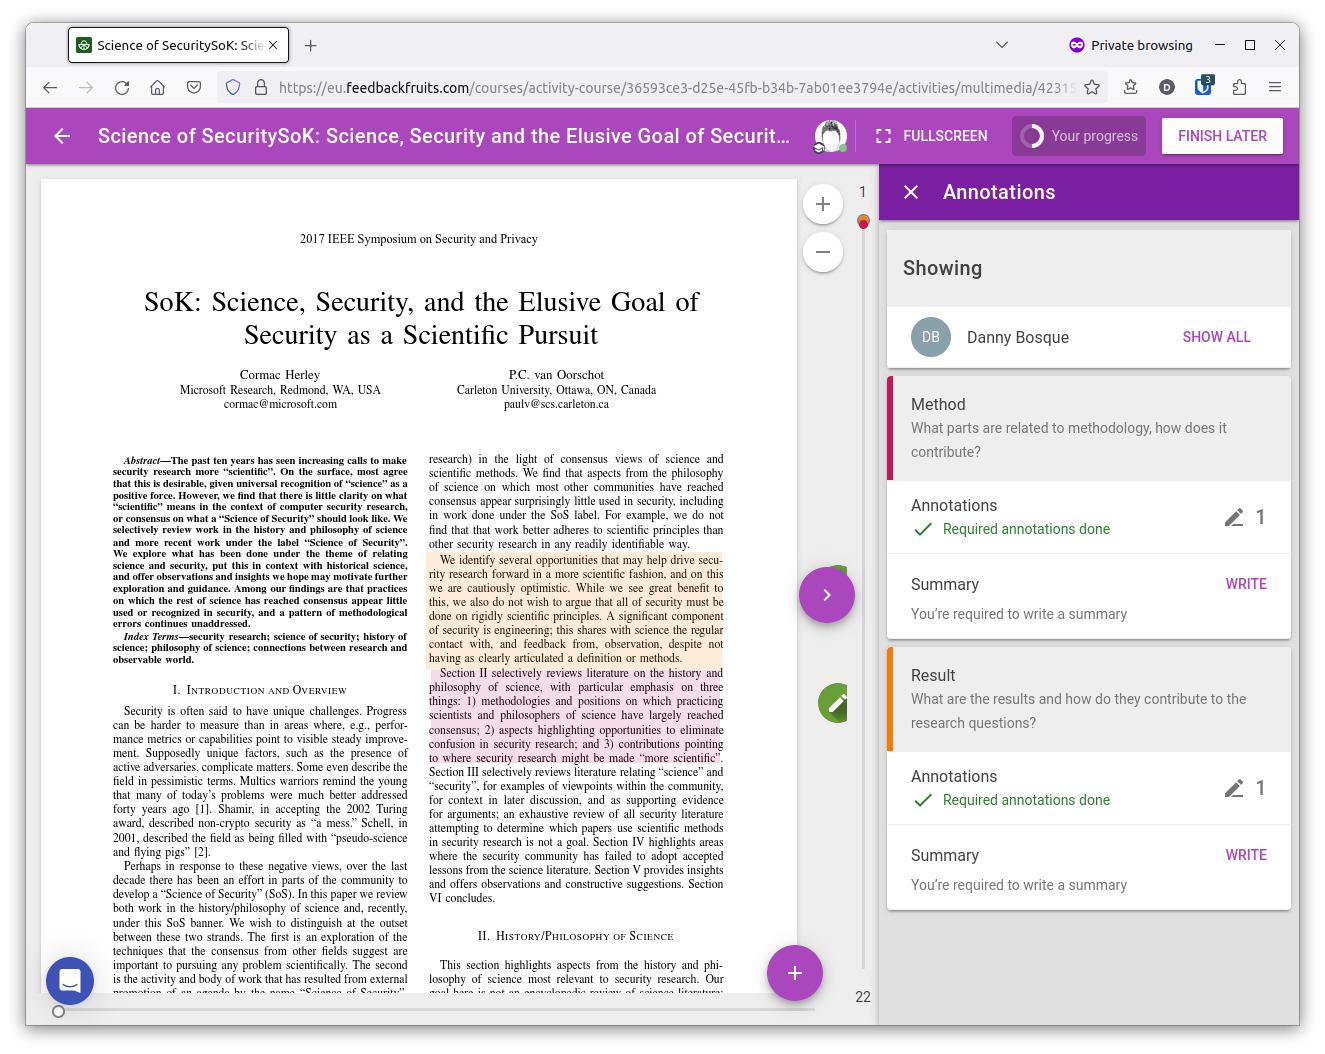
\includegraphics[width=\columnwidth]{figs/fbf-doc-annotations.png}
          \caption{%
            An interactive document in FeedbackFruits where one can annotate 
            the text with focused topics together with other students in the 
            class.%
          }
        \end{figure}
      }
    \end{column}
  \end{columns}
\end{frame}
}

The seminars are used as synchronization points.
The final seminar summarizes the course and results in a grade.

\mode<presentation>{%
\begin{frame}
  \begin{block}{Assessment}
    \begin{itemize}
      \item A synchronous seminar to summarize all work and tie the sack.
    \end{itemize}
  \end{block}
\end{frame}

\begin{frame}
  \begin{block}{Giving the course}
    \begin{enumerate}
      \item Given every period; yes, four times per year.
    \end{enumerate}
  \end{block}
\end{frame}
}

\subsection{Contents}

The course starts with an overview of the complexity.
Then we proceed through a series of \enquote{How do you know it's secure?} case 
studies (assignments mentioned above), that are summarized in two seminars 
(mentioned above).
The idea is to explore how different research methods play together to answer 
different research questions.

\mode<presentation>{%
\begin{frame}
  \begin{block}{Contents}
    \begin{itemize}
      \item Overview of the complexity
    \end{itemize}
    \begin{enumerate}
      \item Purely deductive methods
      \item[\vdots]
      \item[n] Purely inductive methods
    \end{enumerate}
    \begin{itemize}
      \item {Philosophy of Science of Security}
    \end{itemize}
  \end{block}

  \pause

  \begin{remark}[What to focus]
    \begin{itemize}
      \item What does the method contribute?
      \item How do these play together? (Holistic view)
      %\item Emphasize the deduction/induction 
        %divide~\cite{SecurityAsAScience}.
    \end{itemize}
  \end{remark}
\end{frame}
}

We'll try to answer questions like
\enquote{What can deduction possibly say about reality?}
and \enquote{What can induction possibly say about security?}.
And what are the limitations?

\mode<presentation>{%
\begin{frame}
  \begin{example}[Deductive inquiry]
    \begin{itemize}
      \item \enquote{What can deduction possibly say about reality?}
    \end{itemize}
  \end{example}

  \pause

  \begin{example}[Inductive/empirical inquiry]
    \begin{itemize}
      \item \enquote{What can induction possibly say about security?}
    \end{itemize}
  \end{example}

  \pause

  \begin{remark}[To focus on]
    \begin{itemize}
      \item What are the limitations?
      \item Do these require a combination to form a Science of Security?
    \end{itemize}
  \end{remark}
\end{frame}
}

We'll end the teaching part with a seminar more towards the philosophy of 
science of security.
We'll depart in the paper 
\citetitle{SecurityAsAScience}\autocite{SecurityAsAScience} by
\citeauthor{SecurityAsAScience}.

\mode<presentation>{%
\begin{frame}
  \begin{example}[Philosophy of Science of Security]
    \begin{itemize}
      \item Discuss 
        \citetitle{SecurityAsAScience}\footfullcite{SecurityAsAScience}.
      \item What is Science of Security?
      \item Does that even exist at the moment?
      \item Shall we work according to the hypothetico-deductive model?
      \item What are the problems?
    \end{itemize}
  \end{example}
\end{frame}
}

%\begin{frame}
%  \begin{block}{Contents, part II}
%    \begin{itemize}
%      \item General introductions to various subfields.
%      \item Which methods are used and why?
%      \item Some exemplary papers? \alert<2>{Both good and bad!}
%      \item How does a subfield fit into the holistic picture of Security?
%    \end{itemize}
%  \end{block}
%\end{frame}
%
%\begin{frame}
%  \begin{remark}
%    \begin{itemize}
%      \item All above was top down: faculty\footnote{%
%          From different subfields.
%        } present their view on
%        \begin{itemize}
%          \item the methodologies,
%          \item the practices,
%          \item the adversary models,
%          \item the assumptions,
%          \item the relation to scientific approach in their respective 
%            subfield.
%        \end{itemize}
%    \end{itemize}
%  \end{remark}
%\end{frame}
%
%\begin{frame}
%  \begin{block}{Bottom up}
%    \begin{itemize}
%      \item Course participants review the scientific merits of 
%        papers\footnote{%
%          Chosen by subfield designer, not participants.
%        } from top conferences in the subfield.
%
%      \item They identify/reverse engineer methodology and components of 
%        evaluation.
%
%      \item They value why this is scientific and how and what knowledge it 
%        contributes.
%    \end{itemize}
%  \end{block}
%\end{frame}

\subsection{Final assessment}

The final assessment will be an assignment where the students design a research 
method for a given set of research questions.
This will assess all the learning outcomes: \cref{%
  LOrelate,LOcomm,LOplan,LOapply,LOevaluate%
}.

You'll do this by writing a report motivating your choices of methods and 
explaining why they answer the question.
You'll also present this report at the final seminar.
Someone else will review the report, and you will review someone else's report 
too.

The final assessment will be done in pairs.

%\begin{frame}[allowframebreaks]
%  \begin{block}{Assessment}
%    \begin{itemize}
%      \item Apply subfield methodology insights to own paper.
%
%      \item Reflect on how this paper fits in the big picture of Security as a 
%        Science.
%
%      \item Discussion/reflection on limits of how scientific security research 
%        can be; \eg provability versus complexity of actual systems, 
%        engineering versus science.
%
%      \item Peer-review (among course participants) these individual 
%        papers\footnote{%
%          Or a paper in progress or already published paper.
%        } to identify gaps in the scientific approach that could be filled.
%    \end{itemize}
%  \end{block}
%\end{frame}

\begin{frame}<presentation>
  \begin{question}
    \begin{itemize}
      \item Comments, questions, other thoughts?
    \end{itemize}
  \end{question}
\end{frame}


%%% REFERENCES %%%

\begin{frame}[allowframebreaks]
  \only<article>{\printbibliography[heading=bibintoc]}
  \only<presentation>{\printbibliography}
\end{frame}

